\documentclass{article}
\usepackage[a4paper,top=0.75in, bottom=0.75in, left=1in, right=1in,footskip=0.2in]{geometry}
%\usepackage{fullpage}
%-----------------Hyperlink Packages--------------------
\usepackage{hyperref}
\hypersetup{
	 colorlinks   = true,
     citecolor    = black,
     linkcolor    = black,
     urlcolor     = black
}
%-----------------Figure Packages--------------------
\usepackage{graphicx}                       % For figures
%\usepackage{epsfig} % for postscript graphics files
%------------------Math Packages------------------------
\usepackage{amssymb,amsmath}
\usepackage{textcomp}
\usepackage{mdwmath}
\usepackage{mdwtab}
\usepackage{eqparbox}
%------------------Table Packages-----------------------
\usepackage{rotating}                     % Used to rotate tables
\usepackage{array}                        % Fixed column widths for tables
%-----------------Algorithm Packages--------------------
\usepackage{listings}                     % Source code
\usepackage{algorithm}                    % Pseudo Code
\usepackage{algpseudocode}
%---------------------------------------------------------
\usepackage{pgf}
\usepackage{tikz}
\usepackage[utf8]{inputenc}
\usetikzlibrary{arrows,automata}
\usetikzlibrary{positioning}
\usepackage{tikz-qtree,tikz-qtree-compat}

\tikzset{
    state/.style={
           rectangle,
           draw=black,
           minimum height=2em,
           inner sep=2pt,
           text centered,
           },
}

\setcounter{tocdepth}{3}
%opening

\begin{document}

\title{
Course Project for Compilers \\
System Design
}
\author{Class 1, Team 10}
\date{\today}
\maketitle
\tableofcontents
\section{Team Members}

\begin{table}[H]
\centering
\begin{tabular}{l l l}
Name & Student ID  & Job\\
\hline
Fan Ziyao & 12330081 & Team leader, database implementation\\
Chen Zeyu & 12330056 & System implementation \\
Huang Long & 12330132 & Database implementation \\
Zhang Qiuyi (Class 2) & 12330402 & Frontend, documentation \\
Zhu Lichen (Class 2) & 12330439 & Testing
\end{tabular}
\end{table}

\section{System Design}

The system is divided into four parts, with functionalities shown in Figure~\ref{fig:sys}.

The parser doesn't need to concern individual characters, the engine doesn't need to know about tokens and schema/data of tables, and the table doesn't need to know about (raw) statemets. In this way, we make the coupling between modules as loose as possible.

\begin{figure}[H]
\centering
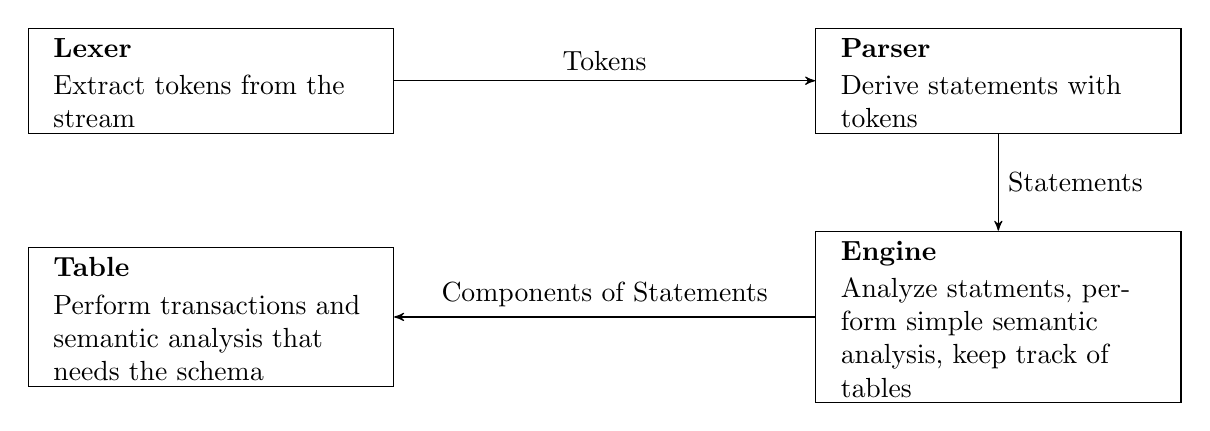
\begin{tikzpicture}[->,>=stealth']

 \node[state, text width=4.5cm] (LEXER) 
 {\begin{tabular}{l}
   \textbf{Lexer}\\[0.3em]
   \parbox{4cm}{Extract tokens from the stream
   }
  \end{tabular}};

 \node[state,
 node distance=10cm,
 text width=4.5cm,
 right of=LEXER,
 ] (PARSER)
 {\begin{tabular}{l}
    \textbf{Parser}\\[0.3em]
    \parbox{4cm}{Derive statements with tokens
    }
   \end{tabular}};
 
 \node[state,
 node distance=3cm,
 text width=4.5cm,
 below of=PARSER,
 ] (ENGINE)
 {\begin{tabular}{l}
     \textbf{Engine}\\[0.3em]
     \parbox{4cm}{Analyze statments,
     perform simple semantic analysis,
     keep track of tables
     }
    \end{tabular}};

 \node[state,
 left of=ENGINE,
 node distance=10cm,
 text width=4.5cm] (TABLE) 
 {\begin{tabular}{l}
      \textbf{Table}\\[0.3em]
      \parbox{4cm}{Perform transactions and
      semantic analysis that needs the schema
      }
     \end{tabular}};


 \path (LEXER) edge node[anchor=east, above]
   {
   	Tokens
   } (PARSER)
   (PARSER) edge node[anchor=east,right]
   {
  	 Statements
   }(ENGINE)
   (ENGINE) edge node[anchor=east,above]
   {
     Components of Statements
   }(TABLE)
 ;
\end{tikzpicture}
\caption{System design}
\label{fig:sys}
\end{figure}

\section{Lexer Design}

\subsection {Token Specification}
\begin{align*}
\text{num}\quad\to\quad & \texttt{[0-9]+} \\
\text{id}\quad\to\quad & \texttt{[\_A-Za-z][\_A-Za-z0-9]*} \\
\text{CREATE}\quad\to\quad & \texttt{CREATE} \\
\text{TABLE}\quad\to\quad & \texttt{TABLE} \\
\text{INT}\quad\to\quad & \texttt{INT} \\
\text{DEFAULT}\quad\to\quad & \texttt{DEFAULT} \\
\text{PRIMARY}\quad\to\quad & \texttt{PRIMARY} \\
\text{KEY}\quad\to\quad & \texttt{KEY} \\
\text{INSERT}\quad\to\quad & \texttt{INSERT} \\
\text{INTO}\quad\to\quad & \texttt{INTO} \\
\text{VALUES}\quad\to\quad & \texttt{VALUES} \\
\text{DELETE}\quad\to\quad & \texttt{DELETE} \\
\text{FROM}\quad\to\quad & \texttt{FROM} \\
\text{WHERE}\quad\to\quad & \texttt{WHERE} \\
\text{SELECT}\quad\to\quad & \texttt{SELECT}
\text{LT}\quad\to\quad & \texttt{<} \\
\text{GT}\quad\to\quad & \texttt{>} \\
\text{NEQ}\quad\to\quad & \texttt{<>} \\
\text{EQ}\quad\to\quad & \texttt{==} \\
\text{GEQ}\quad\to\quad & \texttt{>=} \\
\text{LEQ}\quad\to\quad & \texttt{<=} \\
\text{PLUS}\quad\to\quad & \texttt{+} \\
\text{MINUS}\quad\to\quad & \texttt{-} \\
\text{MUL}\quad\to\quad & \texttt{*} \\
\text{DIV}\quad\to\quad & \texttt{/} \\
\text{AND}\quad\to\quad & \texttt{\&\&} \\
\text{OR}\quad\to\quad & \texttt{||} \\
\text{NOT}\quad\to\quad & \texttt{!} \\
\text{COMMA}\quad\to\quad & \texttt{,} \\
\text{SEMICOLON}\quad\to\quad & \texttt{;} \\
\text{L\_PAREN}\quad\to\quad & \texttt{(} \\
\text{R\_PAREN}\quad\to\quad & \texttt{)}
\end{align*}
\begin{align*}
words \quad\to\quad & \text{CREATE} \quad | \quad \text{TABLE}  \quad | \quad \text{INT} \\
&| \quad \text{DEFAULT} \quad | \quad \text{PRIMARY} \quad | \quad \text{KEY} \quad \\
&| \quad \text{INSERT} \quad | \quad \text{INTO} \quad | \quad \text{VALUES} \quad \\
&| \quad \text{DELETE} \quad | \quad \text{FROM} \quad \\
&| \quad \text{WHERE} \quad | \quad \text{SELECT} \\
singleOp \quad\to\quad &
\text{PLUS} \quad | \quad \text{MINUS} \quad | \quad \text{MUL} \\
&| \quad \text{DIV} \quad | \quad \text{L\_PAREN} \quad | \quad \text{R\_PAREN} \\
&| \quad \text{COMMA} \quad | \quad \text{SEMICOLON} \\
ops \quad\to\quad &
\text{AND} \quad | \quad \text{OR} \quad | \quad \text{NOT} \quad | \quad \text{LT} \\
&| \quad \text{GT} \quad | \quad \text{NEQ} \quad | \quad \text{EQ} \quad | \quad \text{GEQ} \\
&| \quad \text{LEQ} \quad | \quad \text{PLUS} \quad | \quad \text{MINUS} \quad | \quad \text{MUL} \\
&| \quad \text{DIV} \quad | \quad \text{L\_PAREN} \quad | \quad \text{R\_PAREN} \\
&| \quad \text{COMMA} \quad | \quad \text{SEMICOLON}
\end{align*}
\subsection{DFA}

A simplified DFA is shown in Figure~\ref{fig:dfa}. After getting into accepting states for identifiers and operators, we need to further process the buffer to determine the right token to return.

\begin{figure}[H]
\centering
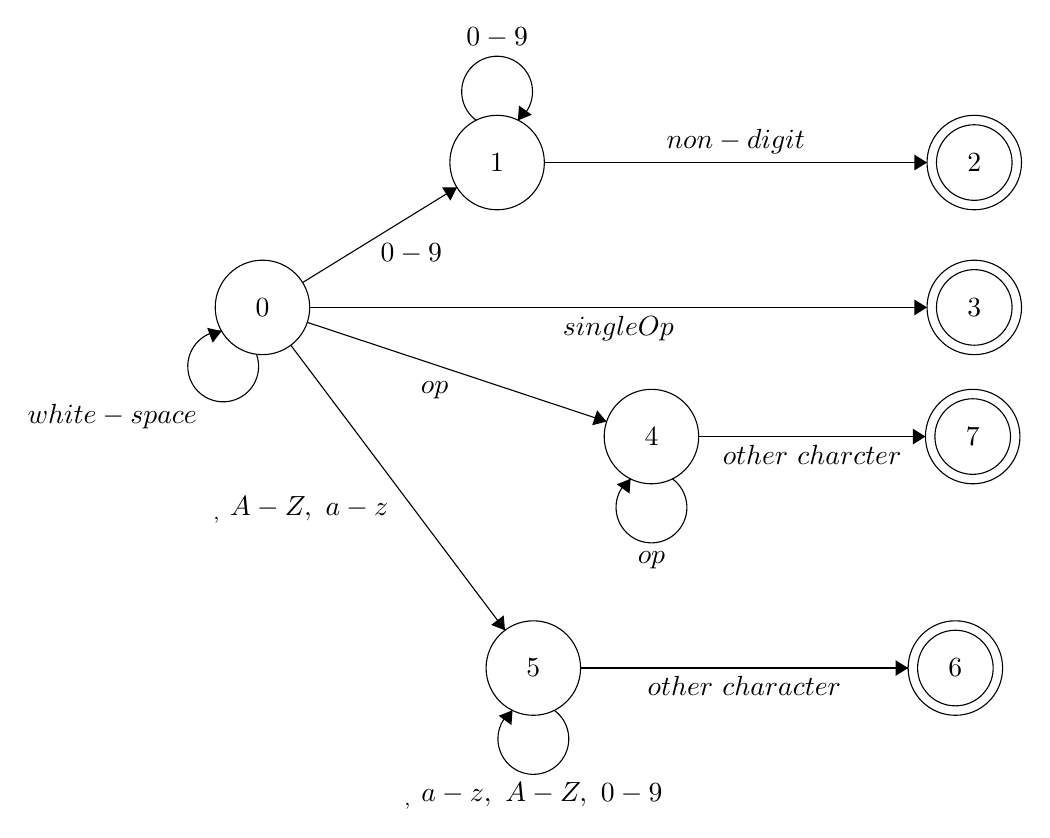
\begin{tikzpicture}[scale=0.2]
\tikzstyle{every node}+=[inner sep=0pt]
\draw [black] (32.8,-10.4) circle (3);
\draw (32.8,-10.4) node {$1$};
\draw [black] (63.1,-10.4) circle (3);
\draw (63.1,-10.4) node {$2$};
\draw [black] (63.1,-10.4) circle (2.4);
\draw [black] (17.9,-19.6) circle (3);
\draw (17.9,-19.6) node {$0$};
\draw [black] (63.1,-19.6) circle (3);
\draw (63.1,-19.6) node {$3$};
\draw [black] (63.1,-19.6) circle (2.4);
\draw [black] (42.6,-27.8) circle (3);
\draw (42.6,-27.8) node {$4$};
\draw [black] (35.1,-42.5) circle (3);
\draw (35.1,-42.5) node {$5$};
\draw [black] (61.9,-42.5) circle (3);
\draw (61.9,-42.5) node {$6$};
\draw [black] (61.9,-42.5) circle (2.4);
\draw [black] (63,-27.8) circle (3);
\draw (63,-27.8) node {$7$};
\draw [black] (63,-27.8) circle (2.4);
\draw [black] (20.45,-18.02) -- (30.25,-11.98);
\fill [black] (30.25,-11.98) -- (29.3,-11.97) -- (29.83,-12.82);
\draw (27.35,-15.5) node [below] {$0-9$};
\draw [black] (35.8,-10.4) -- (60.1,-10.4);
\fill [black] (60.1,-10.4) -- (59.3,-9.9) -- (59.3,-10.9);
\draw (47.95,-9.9) node [above] {$non-digit$};
\draw [black] (31.477,-7.72) arc (234:-54:2.25);
\draw (32.8,-3.15) node [above] {$0-9$};
\fill [black] (34.12,-7.72) -- (35,-7.37) -- (34.19,-6.78);
\draw [black] (17.514,-22.563) arc (20.30993:-267.69007:2.25);
\draw (8.36,-25.72) node [below] {$white-space$};
\fill [black] (15.31,-21.1) -- (14.39,-20.9) -- (14.74,-21.84);
\draw [black] (20.9,-19.6) -- (60.1,-19.6);
\fill [black] (60.1,-19.6) -- (59.3,-19.1) -- (59.3,-20.1);
\draw (40.5,-20.1) node [below] {$singleOp$};
\draw [black] (20.75,-20.55) -- (39.75,-26.85);
\fill [black] (39.75,-26.85) -- (39.15,-26.13) -- (38.84,-27.08);
\draw (28.83,-24.26) node [below] {$op$};
\draw [black] (43.923,-30.48) arc (54:-234:2.25);
\draw (42.6,-35.05) node [below] {$op$};
\fill [black] (41.28,-30.48) -- (40.4,-30.83) -- (41.21,-31.42);
\draw [black] (19.7,-22) -- (33.3,-40.1);
\fill [black] (33.3,-40.1) -- (33.22,-39.16) -- (32.42,-39.76);
\draw (25.92,-32.45) node [left] {$_,\mbox{ }A-Z,\mbox{ }a-z$};
\draw [black] (36.423,-45.18) arc (54:-234:2.25);
\draw (35.1,-49.75) node [below] {$_,\mbox{ }a-z,\mbox{ }A-Z,\mbox{ }0-9$};
\fill [black] (33.78,-45.18) -- (32.9,-45.53) -- (33.71,-46.12);
\draw [black] (38.1,-42.5) -- (58.9,-42.5);
\fill [black] (58.9,-42.5) -- (58.1,-42) -- (58.1,-43);
\draw (48.5,-43) node [below] {$other\mbox{ }character$};
\draw [black] (45.6,-27.8) -- (60,-27.8);
\fill [black] (60,-27.8) -- (59.2,-27.3) -- (59.2,-28.3);
\draw (52.8,-28.3) node [below] {$other\mbox{ }charcter$};
\end{tikzpicture}
\caption{Simplified DFA}
\label{fig:dfa}
\end{figure}

\section{Parser Design}

\subsection{Grammar}

\subsection{\texttt{First} Sets}
\begin{align*}
\textsc{first}(ssql\_stmt) \quad =& \quad\{\text{CREATE, INSERT, DELETE, SELECT}\} \\
\textsc{first}(create\_stmt) \quad =& \quad\{\text{CREATE}\} \\
\textsc{first}(decl\_list) \quad =& \quad\{id\text{, PRIMARY}\} \\
\textsc{first}(\_decl\_list) \quad =& \quad\{\text{COMMA,} \epsilon\} \\
\textsc{first}(decl) \quad =& \quad\{{id\text, PRIMARY}\} \\
\textsc{first}(default\_spec) \quad =& \quad\{\text{DEFAULT,} \epsilon\} \\
\textsc{first}(expr[simple=true]) \quad =& \quad\{\text{PLUS, MINUS, } num \text{, L\_PAREN}\} \\
\textsc{first}(expr[simple=false]) \quad =& \quad\{\text{PLUS, MINUS, }num\text{, }id\} \\
\textsc{first}(\_expr) \quad =& \quad\{\text{PLUS, MINUS, }\epsilon\} \\
\textsc{first}(term[simple=true]) \quad =& \quad\{\text{PLUS, MINUS, }num\text{, L\_PAREN}\} \\
\textsc{first}(term[simple=false]) \quad =& \quad\{\text{PLUS, MINUS, }num\text{, }id\} \\
\textsc{first}(\_term) \quad =& \quad\{\text{MUL, DIV, }\epsilon\} \\
\textsc{first}(unary[simple=true]) \quad =& \quad\{\text{PLUS, MINUS, } num \text{, L\_PAREN}\} \\
\textsc{first}(unary[simple=false]) \quad =& \quad\{\text{PLUS, MINUS, }num\text{, }id\}
%\end{align*}
%\begin{align*}
\textsc{first}(column\_list) \quad =& \quad\{id\} \\
\textsc{first}(\_column\_list) \quad =& \quad\{\text{COMMA, }\epsilon\} \\
\textsc{first}(insert\_stmt) \quad =& \quad\{\text{INSERT}\} \\
\textsc{first}(value\_list) \quad =& \quad\{\text{PLUS, MINUS, } num \text{, L\_PAREN}\} \\
\textsc{first}(\_value\_list) \quad =& \quad\{\text{COMMA, }\epsilon\} \\
\textsc{first}(delete\_stmt) \quad =& \quad\{\text{DELETE}\} \\
\textsc{first}(where\_clause) \quad =& \quad\{\text{WHERE,} \epsilon\} \\
\textsc{first}(disjunct) \quad =& \quad\{\text{L\_PAREN, NOT, PLUS, MINUS, }num\text{, }id\} \\
\textsc{first}(\_disjunct) \quad =& \quad\{\text{OR, }\epsilon\} \\
\textsc{first}(conjunct) \quad =& \quad\{\text{L\_PAREN, NOT, PLUS, MINUS, }num\text{, }id\} \\
\textsc{first}(\_conjunct) \quad =& \quad\{\text{AND, }\epsilon\} \\
\textsc{first}(bool) \quad =& \quad\{\text{L\_PAREN, NOT, PLUS, MINUS, }num\text{, }id\} \\
\textsc{first}(comp) \quad =& \quad\{\text{PLUS, MINUS, }num\text{, }id\} \\
\textsc{first}(rop) \quad =& \quad\{\text{NEQ, EQ, LT, GT, LEQ, GEQ}\} \\
\textsc{first}(query\_stmt) \quad =& \quad\{\text{SELECT}\} \\
\textsc{first}(select\_list) \quad =& \quad\{\text{MUL, }id\} \\
\end{align*}

\subsection{\texttt{Follow} Sets}
\begin{align*}
\textsc{follow}(ssql\_stmt)\quad =& \quad \{\text{\$}\} \\
\textsc{follow}(create\_stmt)\quad =& \quad \{\text{\$}\} \\
\textsc{follow}(decl\_list)\quad =& \quad \{\text{R\_PAREN}\} \\
\textsc{follow}(\_decl\_list)\quad =& \quad \{\text{R\_PAREN}\} \\
\textsc{follow}(decl)\quad =& \quad \{\text{COMMA, R\_PAREN}\} \\
\textsc{follow}(default\_spec)\quad =& \quad \{\text{COMMA, R\_PAREN}\} \\
\textsc{follow}(expr[true])\quad =& \quad \{\text{COMMA, R\_PAREN}\} \\
\textsc{follow}(expr[false])\quad =& \quad \{\text{NEQ, EQ, LT, GT, LEQ,}\\
 & \quad \text{GEQ, AND, OR, SEMICOLON, R\_PAREN}\} \\
\textsc{follow}(\_expr[true])\quad =& \quad \{\text{COMMA, R\_PAREN}\} \\
\textsc{follow}(\_expr[false])\quad =& \quad \{\text{NEQ, EQ, LT, GT, LEQ,}\\
& \quad \text{GEQ, AND, OR, SEMICOLON, R\_PAREN}\} \\
\textsc{follow}(term[true])\quad =& \quad \{\text{PLUS, MINUS, COMMA, R\_PAREN}\} \\
\textsc{follow}(term[false])\quad =& \quad \{\text{PLUS, MINUS, NEQ, EQ, LT, GT,}\\
& \quad \text{LEQ, GEQ, AND, OR, SEMICOLON, R\_PAREN}\} \\
\textsc{follow}(\_term[true])\quad =& \quad \{\text{PLUS, MINUS, COMMA, R\_PAREN}\} \\
\textsc{follow}(\_term[false])\quad =& \quad \{\text{PLUS, MINUS, NEQ, EQ, LT, GT,}\\
& \quad \text{LEQ, GEQ, AND, OR, SEMICOLON, R\_PAREN}\} \\
\textsc{follow}(unary[true])\quad =& \quad \{\text{MUL, DIV, PLUS, MINUS, COMMA, R\_PAREN}\} \\
\textsc{follow}(unary[false])\quad =& \quad \{\text{MUL, DIV, PLUS, MINUS, NEQ, EQ, LT,} \\
& \quad \text{GT, LEQ, GEQ, AND, OR, SEMICOLON, R\_PAREN}\} 
%\end{align*}
%\begin{align*}
\textsc{follow}(column\_list)\quad =& \quad \{\text{FROM, R\_PAREN}\} \\
\textsc{follow}(\_column\_list)\quad =& \quad \{\text{FROM, R\_PAREN}\} \\
\textsc{follow}(insert\_stmt)\quad =& \quad \{\text{\$}\} \\
\textsc{follow}(value\_list)\quad =& \quad \{\text{R\_PAREN}\} \\
\textsc{follow}(\_value\_list)\quad =& \quad \{\text{R\_PAREN}\} \\
\textsc{follow}(delete\_stmt)\quad =& \quad \{\text{\$}\} \\
\textsc{follow}(where\_clause)\quad =& \quad \{\text{SEMICOLON}\} \\
\textsc{follow}(disjunct)\quad =& \quad \{\text{SEMICOLON, R\_PAREN}\} \\
\textsc{follow}(\_disjunct)\quad =& \quad \{\text{SEMICOLON, R\_PAREN}\} \\
\textsc{follow}(conjunct)\quad =& \quad \{\text{OR, SEMICOLON, R\_PAREN}\} \\
\textsc{follow}(\_conjunct)\quad =& \quad \{\text{OR, SEMICOLON, R\_PAREN}\} \\
\textsc{follow}(bool)\quad =& \quad \{\text{AND, OR, SEMICOLON, R\_PAREN}\} \\
\textsc{follow}(comp)\quad =& \quad \{\text{AND, OR, SEMICOLON, R\_PAREN}\} \\
\textsc{follow}(rop)\quad =& \quad \{\text{PLUS, MINUS, }num \text{, } id\} \\
\textsc{follow}(query\_stmt)\quad =& \quad \{\text{\$}\} \\
\textsc{follow}(select\_list)\quad =& \quad \{\text{FROM}\} 
\end{align*}
\subsection{Parsing Table}

Format:
\begin{align*}
\text{Current production} \quad  \to & \quad\\
\text{Lookahead}: & \quad \text{Production body to match}
\end{align*}

For simplicity, we combine $simple\_expr$ and $expr$ into $expr[simple]$, distinguished by $expr[true]$ and $expr[false]$.

\begin{align*}
ssql\_stmt \quad  \to & \quad\\
\text{CREATE}: & \quad create\_stmt \\
\text{INSERT}: & \quad insert\_stmt \\
\text{DELETE}: &  \quad delete\_stmt \\
\text{SELECT}: & \quad query\_stmt
\end{align*}

\begin{align*}
create\_stmt \quad  \to & \quad\\
\text{CREATE:} & \quad \text{CREATE TABLE } id \text{ L\_PAREN } decl\_list \text{ R\_PAREN SEMICOLON}
\end{align*}

\begin{align*}
decl\_list \quad  \to & \quad\\
id: & \quad decl\text{ }\_decl\_list \\
\text{PRIMARY}: & \quad decl\text{ }\_decl\_list
\end{align*}

\begin{align*}
\_decl\_list \quad  \to & \quad\\
\text{COMMA}: & \quad \text{COMMA } decl\text{ }\_decl\_list \\
\text{R\_PAREN}: & \quad \epsilon
\end{align*}

\begin{align*}
decl \quad  \to & \quad\\
id: & \quad id \text{ INT } default\_spec \\
\text{PRIMARY}: & \quad \text{PRIMARY KEY L\_PAREN }column\_list \text{ R\_PAREN}
\end{align*}

\begin{align*}
default\_spec \quad  \to & \quad\\
\text{DEFAULT}: & \quad \text{DEFAULT ASSIGN } expr[true] \\
\text{COMMA}: & \quad \epsilon \\
\text{R\_PAREN}: & \quad \epsilon
\end{align*}

\begin{align*}
column\_list \quad  \to & \quad\\
id: & \quad id \text{ } \_column\_list
\end{align*}


\begin{align*}
\_column\_list \quad  \to & \quad\\
\text{COMMA}: & \quad \text{COMMA } id \text{ } \_column\_list \\
\text{FROM}: & \quad \epsilon \\
\text{R\_PAREN}: & \quad \epsilon
\end{align*}

\begin{align*}
insert\_stmt \quad  \to & \quad\\
\text{INSERT}: & \quad \text{INSERT INTO } id \text{ L\_PAREN } column\_list \text{ R\_PAREN} \\
& \quad \text{VALUES L\_PAREN } value\_list \text{ R\_PAREN SEMICOLON}
\end{align*}

\begin{align*}
value\_list \quad  \to & \quad\\
\text{PLUS}: & \quad expr[true] \text{ } \_value\_list \\
\text{MINUS}: & \quad expr[true] \text{ } \_value\_list \\
num: & \quad expr[true] \text{ } \_value\_list \\
\text{L\_PAREN}: & \quad expr[true] \text{ } \_value\_list
\end{align*}

\begin{align*}
\_value\_list \quad  \to & \quad\\
\text{COMMA}: & \quad \text{COMMA } expr[true] \text{ } \_value\_list \\
\text{R\_PAREN}: & \quad \epsilon
\end{align*}

\begin{align*}
delete\_stmt \quad  \to & \quad\\
\text{DELETE}: & \quad \text{DELETE FROM } id \text{ } where\_clause \text{ SEMICOLON}
\end{align*}


\begin{align*}
disjunct \quad  \to & \quad\\
\text{L\_PAREN}: & \quad conjunct \text{ } \_disjunct \\
\text{NOT}: & \quad conjunct \text{ } \_disjunct \\
\text{PLUS}: & \quad conjunct \text{ } \_disjunct \\
\text{MINUS}: & \quad conjunct \text{ } \_disjunct \\
num: & \quad conjunct \text{ } \_disjunct \\
id: & \quad conjunct \text{ } \_disjunct
\end{align*}

\begin{align*}
\_disjunct \quad  \to & \quad\\
\text{OR}: & \quad \text{OR } conjunct \text{ } \_disjunct\\
\text{SEMICOLON}: & \quad \epsilon \\
\text{R\_PAREN}: & \quad \epsilon
\end{align*}

\begin{align*}
conjunct \quad  \to & \quad\\
\text{L\_PAREN}: & \quad bool \text{ } \_conjunct \\
\text{NOT}: & \quad bool \text{ } \_conjunct \\
\text{PLUS}: & \quad bool \text{ } \_conjunct \\
\text{MINUS}: & \quad bool \text{ } \_conjunct \\
num: & \quad bool \text{ } \_conjunct \\
id: & \quad  bool \text{ } \_conjunct
\end{align*}

\begin{align*}
\_conjunct \quad  \to & \quad\\
\text{AND}: & \quad \text{AND } bool \text{ } \_conjunct\\
\text{OR}: & \quad \epsilon \\
\text{SEMICOLON}: & \quad \epsilon \\
\text{R\_PAREN}: & \quad \epsilon
\end{align*}

\begin{align*}
bool \quad  \to & \quad\\
\text{L\_PAREN}: & \quad \text{L\_PAREN } disjunct \text{ R\_PAREN} \\
\text{NOT}: & \quad \text{NOT } bool \\
\text{PLUS}: & \quad comp \\
\text{MINUS}: & \quad comp \\
num: & \quad comp \\
id: & \quad comp
\end{align*}

\begin{align*}
comp \quad  \to & \quad\\
\text{PLUS}: & \quad expr[false] \text{ } rop  \text{ } expr[false] \\
\text{MINUS}: & \quad expr[false] \text{ } rop  \text{ } expr[false] \\
num: & \quad expr[false] \text{ } rop  \text{ } expr[false] \\
id: & \quad expr[false] \text{ } rop  \text{ } expr[false]
\end{align*}

Here things like $term[simple]$ means passing down the current value $simple$.

\begin{align*}
expr[simple] \quad  \to & \quad\\
\text{PLUS}: & \quad term[simple] \text{ } \_expr[simple] \\
\text{MINUS}: & \quad term[simple] \text{ } \_expr[simple] \\
num: & \quad term[simple] \text{ } \_expr[simple] \\
if (simple == false): &\\
\text{L\_PAREN}: & \quad term[simple] \text{ } \_expr[simple] \\
if (simple == true): &\\
id: & \quad term[simple] \text{ } \_expr[simple] 
\end{align*}

\begin{align*}
\_expr[simple] \quad  \to & \quad\\
\text{PLUS}: &\quad \text{PLUS }  term[simple] \text{ } \_expr[simple] \\
\text{MINUS}: &\quad \text{MINUS }  term[simple] \text{ } \_expr[simple] \\
if (simple == true): &\\
\text{COMMA} : & \quad \epsilon \\
\text{R\_PAREN} : & \quad \epsilon \\
if (simple == true): &\\
\text{NEQ} : & \quad \epsilon \\
\text{EQ} : & \quad \epsilon \\
\text{LT} : & \quad \epsilon \\
\text{GT} : & \quad \epsilon \\
\text{LEQ} : & \quad \epsilon \\
\text{GEQ} : & \quad \epsilon \\
\text{AND} : & \quad \epsilon \\
\text{OR} : & \quad \epsilon \\
\text{SEMICOLON} : & \quad \epsilon \\
\text{R\_PAREN} :  & \quad \epsilon
\end{align*}

\begin{align*}
term[simple] \quad  \to & \quad\\
\text{PLUS}: & \quad unary[simple] \text{ } \_term[simple] \\
\text{MINUS}: & \quad unary[simple] \text{ } \_term[simple] \\
num: & \quad unary[simple] \text{ } \_term[simple] \\
if (simple == false): &\\
\text{L\_PAREN}: & \quad unary[simple] \text{ } \_term[simple] \\
if (simple == true): &\\
id: & \quad unary[simple] \text{ } \_term[simple] 
\end{align*}

\begin{align*}
\_term[simple] \quad  \to & \quad\\
\text{MUL}: &\quad \text{MUL }  unary[simple] \text{ } \_term[simple] \\
\text{DIV}: &\quad \text{DIV }  unary[simple] \text{ } \_term[simple] \\
if (simple == true): &\\
\text{COMMA} : & \quad \epsilon \\
\text{R\_PAREN} : & \quad \epsilon \\
if (simple == true): &\\
\text{NEQ} : & \quad \epsilon \\
\text{EQ} : & \quad \epsilon \\
\text{LT} : & \quad \epsilon \\
\text{GT} : & \quad \epsilon \\
\text{LEQ} : & \quad \epsilon \\
\text{GEQ} : & \quad \epsilon \\
\text{AND} : & \quad \epsilon \\
\text{OR} : & \quad \epsilon \\
\text{SEMICOLON} : & \quad \epsilon \\
\text{R\_PAREN} :  & \quad \epsilon
\end{align*}

\begin{align*}
unary[simple] \quad  \to & \quad\\
\text{PLUS}: & \quad \text{PLUS } unary[simple]\\
\text{MINUS}: & \quad \text{MINUS } unary[simple]\\
num: & \quad num \\
if (simple == false): &\\
\text{L\_PAREN}: & \quad \text{L\_PRAEN } expr[true] \text{ R\_PRAEN}\\
if (simple == true): &\\
id: & \quad id
\end{align*}

\begin{align*}
rop \quad  \to & \quad\\
\text{NEQ} : & \quad \text{NEQ} \\
\text{EQ} : & \quad \text{EQ} \\
\text{LT} : & \quad \text{LT} \\
\text{GT} : & \quad \text{GT} \\
\text{LEQ} : & \quad \text{LEQ} \\
\text{GEQ} : & \quad \text{GEQ}
\end{align*}

\begin{align*}
query\_stmt \quad  \to & \quad\\
\text{SELECT}: & \quad \text{SELECT } select\_list \text{ FROM } id \text{ } where\_clause \text{ SEMICOLON}
\end{align*}

\begin{align*}
select\_list \quad  \to & \quad\\
\text{MUL}: & \quad \text{MUL} \\
id: & \quad column\_list
\end{align*}

\subsection{About expressions}

To handle expressions, we build expression trees during parsing, then attach them to statements as a component for later evaluation(in-order). An example is shown in Figure~\ref{fig:tree}.

\begin{figure}[H]
\centering
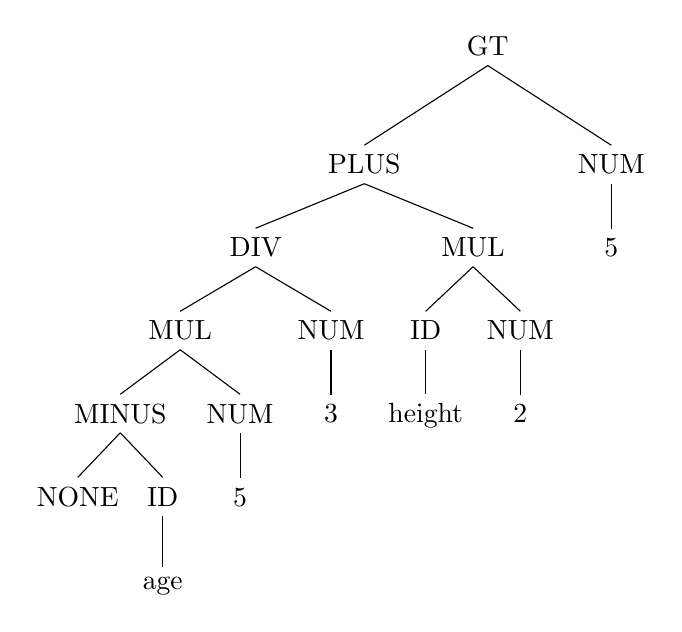
\begin{tikzpicture}[level 1/.style={level distance=1.5cm}]
\Tree
[.GT
  [.PLUS
    [.DIV [.MUL [.MINUS [.NONE   ] [.ID age ] ] [.NUM 5 ] ] [.NUM 3 ] ] 
    [.MUL [.ID height ] [.NUM 2 ] ]
  ] 
  [.NUM 5 ]
]
\end{tikzpicture}
\caption{Expression tree for $-age * 5 / 3 + height * 2 > 5$}
\label{fig:tree}
\end{figure}

\subsection{Statements}
During parsing, we collect items for list-type components in statements. For example, when parsing a column list, we pass a vector around,  pushing $id$s into it each time a terminal $id$ is consumed. Similarly, default specifications for a $Create$ statement is a map from strings to int, value list is a vector of int, etc. In this way, we can completely seperate the parser from the table.

\section{Database Design}

As shown in Figure~\ref{fig:db}, we divide the backend into two parts: engine and table.

Engine is responsible for inter-table operations. It receives statements produced by the parser, performs basic semantic analysis(those that can be done without knowing the data or schema in any table), and keeps track of tables in the memory. Engine can extract legal components inside statements (e.g. a vector of primary keys in a $Create$ statement), and pass it down to the right table to perform transactions.

Table is responsible for intra-table operations. It receives components of statements from the engine, performs semantic analysis that needs the knowledge of its data and schema, and finishes transactions.

Both engine and table provide services for creating tables, inserting records, deleting records and querying records, though at different levels.

\begin{figure}[H]
\centering
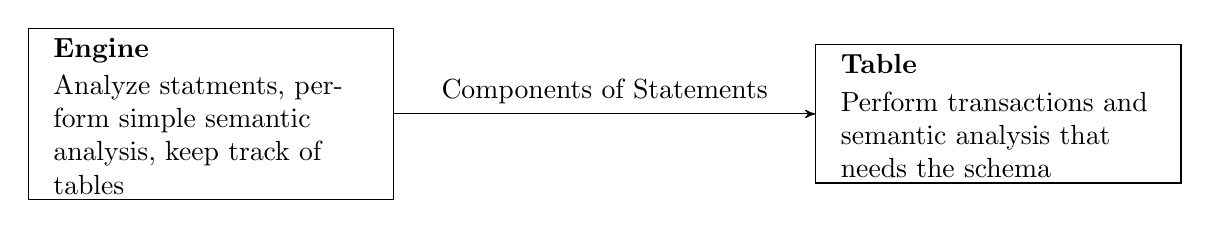
\begin{tikzpicture}[->,>=stealth']
 \node[state,
 node distance=3cm,
 text width=4.5cm,
 ] (ENGINE)
 {\begin{tabular}{l}
     \textbf{Engine}\\[0.3em]
     \parbox{4cm}{Analyze statments,
     perform simple semantic analysis,
     keep track of tables
     }
    \end{tabular}};

 \node[state,
 right of=ENGINE,
 node distance=10cm,
 text width=4.5cm] (TABLE) 
 {\begin{tabular}{l}
      \textbf{Table}\\[0.3em]
      \parbox{4cm}{Perform transactions and
      semantic analysis that needs the schema
      }
     \end{tabular}};

 \path (ENGINE) edge node[anchor=west,above]
   {
     Components of Statements
   }(TABLE)
 ;
\end{tikzpicture}
\caption{Database Design}
\label{fig:db}
\end{figure}

\subsection{Error Recovery}

For errors ocurred during lexical analysis, if the invalid lexeme appears as a start symbol, we stop the program since this can lead to numerous parse errors. Otherwise we simply igonre this lexeme, and ignore the whole statement if necessary.

For parse errors, runtime errors(division by zero, column can't be found in the schema) and database errors, we skip to the next start symbol, and parse the next statement.

\section{Complexity Analysis}

Our implementation of the lexer is rather simple. It only needs to backtrack when matching operators that can be a prefix of another operator(e.g. $<$ and $<=$). Since in this language the length of an operator is no more than 2, the overhead of the backracking can be ignored.

For this context-free grammar, we implement a LL(1) predictive parser. The overhead is also negligible.

Since it is not a database course, we implement the backend in a naive way. The data is stored unsorted in a 2-dimensional vector of ints.

The creation of tables has a negligible overhead when there are just a few tables in the database. The other three operations, however, has a bigger overhead because of the naive implementation. Assume that a table has $k$ columns, $N$ records, the complexity of insertion is about $O(Nk)$ since we need to check key constraints against every record. For a where clause containing an expression with $E$ operations, deleting a record costs about $O(NE)$, querying a record costs about $O(NEk)$ ($O(NE)$ if no reordering is needed). Again, this is not a database course, so we didn't build any special indexes for it. This performance is sufficient for testing our implementation of the language.

\end{document}
